% Общий объем раздела 25-30 стр.

\section{Разработка и реализация алгоритмов стегоанализа изображений с использованием свёрточных искусственных нейронных сетей}

Широкое распространение стегоаналитических подходов, использующих МОВ, дало мощный толчок появлению стеганографических систем с большей стегоскрытностью, что в свою очередь дало старт росту размерности пространства признаков, формируемого стегоаналитиком. Ручное конструирование сотен признаков --- трудоёмкая задача, что стало одной из причин появления стегоаналитических алгоритмов с использованием свёрточных искусственных нейронных сетей.

\subsection{Описание нейросетевого подхода и общей схемы алгоритма}

Одной из первых работ, положивших начало нейросетевому подходу к решению задач классификации, стало изобретение линейного перцептрона Фрэнком Розенблаттом~\cite{Rosenblatt1, Rosenblatt2}. По сути своей перцептрон Розенблатта --- это линейная модель бинарной классификации, задача которой --- научиться сопоставлять метки классов не участвовавшим в обучении объектам.

Будем считать, что каждый вход представляет собой вектор вещественных чисел $ x = (x_1, x_2, \ldots, x_d) \in \mathbb{R}^d $, и входы в тренировочном множестве снабжены известными выходами $ y(\mathbf{x}) \in \{-1, 1\} $. Тогда для решения задачи необходимо найти такие веса $ w_0, w_1, \ldots, w_d \in \mathbb{R}^d $, чтобы знак линейной функции
\begin{equation*}
sign(w_0 + w_1x_1 + w_2x_2 + \ldots + w_dx_d)
\end{equation*}
как можно чаще совпадал с правильным ответом $ y(x) $. Для удобства увеличим размерность вектора $ x $ таким образом, чтобы он принял вид $ x = (1, x_1, x_2, \ldots, x_d) \in \mathbb{R}^{d + 1} $. Это позволит считать линейную комбинацию $ w_0 + w_1x_1 + w_2x_2 + \ldots + w_dx_d $ скалярным произведением $ \mathbf{w}^T\mathbf{x} $, где $ \mathbf{w} = (w_0, w_1, w_2, \ldots, w_d) $. Часто $ w_0 $ также обозначают как $ b $ и называют смещением, т. к. этот коэффициент выполняет смещение, когда х = 0.

Для обучения данной функции необходимо выбрать функцию ошибки. Розенблатт вводит в этом качестве \textit{критерий перцептрона}:
\begin{equation}
E_P(\mathbf{w}) = - \sum_{x \in \mathbb{M}} y(\mathbf{x})(\mathbf{w}^T\mathbf{x}),
\label{eq:PerceptronCriterion}
\end{equation}
где $ \mathbb{M} $ обозначает множество множество примеров, которые перцептрон с весами $ \mathbf{w} $ классифицирует неверно.

Оптимизировать~\ref{eq:PerceptronCriterion} можно методом градиентного спуска. На очередном шаге обучения~$ \tau $ получим:
\begin{equation*}
\mathbf{w}^{(\tau + 1)} = \mathbf{w}^{(\tau)} - \eta\nabla_{\mathbf{w}}E_P(\mathbf{w}) = \mathbf{w}^{(\tau)} + {\eta}t_nx_n.
\end{equation*}

Такой линейный классификатор способен решать только элементарные задачи с линейно разделимыми выборками. Для построения на основе перцептрона Розенблатта нелинейного классификатора применяют нелинейную функцию активации, принимающую на вход линейную комбинацию $ \mathbf{w}^T\mathbf{x} $. Наиболее популярная исторически функция активации --- \textit{логистический сигмоид}:
\begin{equation*}
f(x) = \frac{1}{1 + e^{-x}}.
\end{equation*}

Как и другие функции активации нейронов, это монотонно неубывающая функция, которая при $ x \to -\infty $ стремится к нулю, а при $ x \to +\infty $~--- к единице. Это значит, что при подаче на вход большого по модулю отрицательного числа нейрон не активируется, а при подаче такого же положительного --- активируется почти наверняка.

Введение данной функции активации вкупе с переобозначением меток классов: $ -1 \to 0 $, $ +1 \to 1 $ и исползованием перекрёстной энтропии
\begin{equation*}
E(\mathbf(w) = -\frac{1}{N}\sum_{i = 1}{N} (y_ilog(f(\mathbf{w}^T\mathbf{x}_i)) + (1 - y_i)log(1 - f(\mathbf{w}^T\mathbf{x}_i)).
\end{equation*}
в качестве функции ошибок позволяет решать задачу логистической регрессии, что позволяет интерпретировать $ y(\mathbf{x}) $ как вектор вероятностей.

Перейдём от одного нейрона к нейронной сети. Обозначим выход $ j $\=/того нейрона $ l $\=/того слоя как $ y_j^l $:
\begin{equation*}
y_j^l = f(\sum_k w_{jk}^ly_k^{l - 1} + b_j^l),
\end{equation*}
а в качестве функции активации последнего слоя выберем \textit{softmax}.

В данном случае для минимизации значения функции ошибок необходимо подобрать параметры уже не одного нейрона, а всей сети. Для этого используется метод обратного распространения ошибки, являющийся модификацией метода градиентного спуска. В качестве функции ошибок преимущественно используется категориальная перекрёстная энтропия.

\subsubsection{Обзор архитектуры свёрточной нейронной сети}

Свёрточная нейронная сеть состоит из одного или нескольких свёрточных слоёв, предшествующих нескольким полносвязным слоям нейронов, аналогичным классическим многослойным нейронным сетям прямого распространения. Основная идея свёрточных слоёв заключается в извлечении из двумерных матриц наборов карт признаков, которые могли бы позволить классификатору получить лучшее представление оригинальных данных. С одной стороны, они уменьшают размерность входа, с другой~--- автоматически выделяют наиболее существенные признаки входных данных. Это объясняет успех свёрточных нейронных сетей в области распознавания образов и классификации изображений.


\begin{figure}
\centering
\includegraphics[width=1\textwidth]{include/graphics/cnn_architecture_example}
\caption{Архитектура GNCNN}
\label{fig:GNCNNArchitecture}
\end{figure}


Каждый свёрточный слой обычно выполняет три операции для получения карт признаков. Первый шаг --- фильтрация методом скользящего окна с использованием $ K $ ядер, результатом которой является $ K $ карт признаков. Каждое ядро применяется к существующей карте признаков, полученной в предыдущем слое. В первом свёрточном слое все ядра применяются к исходному изображению. Затем производится уменьшение размерности карт признаков с помощью операции субдискретизации (пулинга) путём вычисления среднего или максимального значения в каждом регионе карты признаков размера $ p \times p $. Финальный шаг --- расчёт нелинейной функции карты признаков.

В сравнении с полносвязными слоями свёрточные слои обучаются быстрее ввиду использования метода скользящего окна. Благодаря этому, в обучении нуждаются не все связи между соседними слоями, а только элементы свёрточного ядра, общего для одной конкретной матрицы. Это разделение весов не только существенно уменьшает их количество, но и повышает обобщающие способности сети, позволяя формировать универсальные относительно различных участков изображений свёрточные ядра.

Как и в нейронных сетях других типов, процесс обучения заключается в минимизации функции потерь с использованием оптимизационного алгоритма, обновляющего веса. Пакетный режим стохастического градиентного спуска в качестве оптимизационного алгоритма очень популярен, но AdaDelta или AdaGrad также могут применятся в свёрточных нейронных сетях. 

Рассмотрим детальнее некоторые операции, применяемые в свёрточных слоях.

\textbf{Свёртка.} Обозначим результат свёртки в слое $ l $ с $ k $\=/ым ядром, равным матрице весов $ W^{kl} $, как $ C^{kl} $. Тогда
\begin{equation*}
C^{kl} = \sum_{m = 1}^{K^{l - 1}} (W^{kl} * F^{m(l - 1)}),
\end{equation*}
где $ * $ обозначает операцию свёртки. $ K^{l - 1} $~--- это количество ядер в предыдущем слое, а $ F^{m(l - 1)} $~--- $ k $\=/ая карта признаков, полученная из предыдущего слоя. Для первого свёрточного слоя $ l = 1 $, $ K^{l - 1} = K^0 = 1 $, а $ F^{1(l - 1)} = F^{10} = I $, где $ I $~--- входное изображение. Размер матрицы фильтрации $ W^{kl} $ напрямую определяет размер локальной области (скользящего окна), используемой для вычисления $ C^{kl}_{ij} $.

Размер выходной матрицы также зависит от двух параметров, называемых шагом свёртки и дополнением (англ.~padding). Шаг свёртки $ S $ задаёт дискрет перемещения скользящего окна, регулирующий степень пересечения локальных областей. Дополнение позволяет дополнить входную карту признаков $ F^{m(l - 1)} $ или изображение $ I $ нулями по краям. Обозначим толщину дополнения $ P $.

\begin{equation*}
dim(C^{kl}) = (dim(F^{m(l - 1)}) - dim(W^{kl}) + 2 \times P) / S + 1.
\end{equation*}

Например, для сохранения размерности $ C^{kl} $ равной размерности входных данных $ F^{m(l - 1)} $ ($ dim(C^{kl}) = dim(F^{m(l - 1)} $) необходимо соблюсти условие
\begin{equation*}
\begin{cases}
S = 1, \\
P = dim(W^{kl}/2). \\
\end{cases}
\end{equation*}

\textbf{Функция активации.} Для внесения нелинейности каждый результат свёртки $ C^{kl} $ обрабатывается с помощью функции активации $ f^{kl}: \mathbb{R} \to \mathbb{R} $ так же, как это происходит в других типах нейронных сетей. В качестве функции активации в свёрточных нейронных сетях часто используются логистический сигмоид, гиперболический тангенс $ f(x) = tanh(x) $ и ReLU:
\begin{equation*}
f(x) = max(0, x).
\end{equation*}

\textbf{Субдискретизация (пулинг).} Результатом применения данной операции является уменьшение размерности двумерного массива путём его разбиения на фрагменты размером $ p_l \times p_l $ с последующей заменой каждого фрагмента средним или максимальным значением его элементов. Значение шага регулирует пересечение соседних фрагментов, хотя наиболее часто шагу присваивается значение $ p_l $, и пересечения не происходит. Значение $ p_l $ обычно выбирается в диапазоне от 2 до 5, в зависимости от размерности входных данных слоя $ l $.

Субдискретизация выполняет две функции: на уровне одного слоя --- снижение размерности и путём вычисления «типичного» признака фрагмента или взятия наиболее сильно проявляющегося признака; на уровне сети в целом --- агрегирование низкоуровневых признаков в высокоуровневые.

В задачах стегоанализа выбор операции усреднения при осуществлении субдискретизации оправдан слабым характером стеговоздействия, не позволяющим ему достаточно часто принимать максимальное значение на карте признаков.

Запишем выражение для выхода первого свёрточного слоя:
\begin{align*}
F^{k1} &= pooling(f^{k1}(\sum_{m = 1}^{K^0}(W^{k1} * F^{m(l - 1)}) + b^{k1})) = pooling(f^{k1}(W^{k1}*F^{10} + b^{k1})) \\
&= pooling(f^{k1}(W^{k1} * I + b^{k1})).
\end{align*}

\subsection{Свёрточная нейронная сеть GNCNN}

Модель свёрточной нейронной сети для стегоанализа изображений в оттенках серого GNCNN была предложена в~\cite{GNCNN}. Её основные отличительные особенности: применение фильтра предварительной обработки и использование функции Гаусса в качестве функции активации нейронов свёрточных слоёв.
\begin{equation}
\label{eq:GNCNNConvKernel}
%\begin{align*}
K = \frac{1}{12}
\begin{pmatrix*}[r]
    -1 &  2 &    -2 &  2 & -1 \\
     2 & -6 &     8 & -6 &  2 \\
    -2 &  8 & -12 &  8 & -2 \\
     2 & -6 &     8 & -6 &  2 \\
    -1 &  2 &    -2 &  2 & -1 \\
\end{pmatrix*}
%\end{align*}
\end{equation}

Полосовой высокочастотный фильтр предварительной обработки с импульсной характеристикой~\eqref{eq:GNCNNConvKernel} введён исходя из априорного знания о слабом характере стеговоздействия на стегоконтейнер. Целью предварительной фильтрации является усиление яркости стегосигнала и ослабление яркости оригинального изображения. Веса данного фильтра заранее предопределены и не участвуют в процессе обучения нейронной сети.

Ещё одним преобразованием, облегчающим процесс извлечения признаков, является переход от оригинального изображения к шумоподобному остатку $ R = (r_{ij}) $, содержащему только предсказания относительно факта стеганографической модификации каждого пикселя:
\begin{equation*}
r_{ij} = y_{ij} - P(N(Y, i, j)),
\end{equation*}
где $ Y = (y_{ij}) $ – стегоконтейнер, а $ P(N(Y, i, j)) $ – оценка значения пикселя $ y_{ij} $, полученная из окружающих его пикселей $ N(Y, i, j) $~\cite{FridrichNoiseResidual}. Ввиду наличия сложных зависимостей между соседними пикселями, в случае отсутствия модификации оценка зачастую будет близка к действительному значению пикселя $ y_{ij} $, а значение $ r_{ij} $ будет близко к нулю.
\begin{equation}
\label{eq:GaussianFunction}
%\begin{align*}
f(x) = e^{-\frac{x^2}{\sigma^2}}
%\end{align*}
\end{equation}

Функция Гаусса~\eqref{eq:GaussianFunction} с нулевым математическим ожиданием в качестве функции активации (рис.~\ref{fig:GaussianFunction}) призвана обеспечить формирование в свёрточном слое нейронной сети такого ядра $ K $, что $ Y*K = R $. Максимальное значение функции в нуле соответствует нулевой ошибке оценки значения $ y_{ij} $ и, следовательно, предположению об отсутствии модификации пикселя стегоконтейнера. Резкий спад по мере удаления от нуля обращает в близкие к нулю значения любой результат свёртки, превышающий порог, определяемый среднеквадратическим отклонением $ \sigma $, влияющим на ширину кривой.

\begin{figure}
\centering
\includegraphics[width=1\textwidth]{include/graphics/gaussian_function}
\caption{Функция активации GNCNN}
\label{fig:GaussianFunction}
\end{figure}

Архитектура нейронной сети представлена на рис.~\ref{fig:GNCNNArchitecture} и имеет вид состояний, через которые проходит входное изображение. Между состояниями располагаются порядковые номера слоёв.

\begin{figure}
\centering
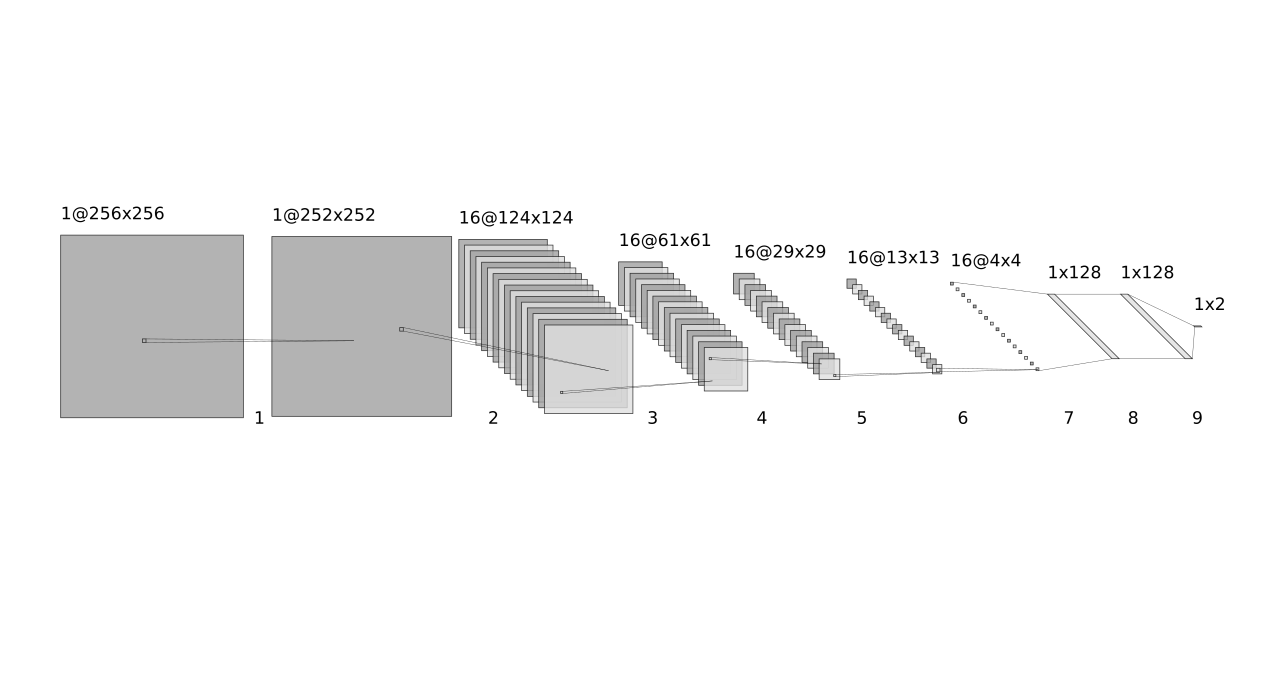
\includegraphics[width=1\textwidth]{include/graphics/gncnn_gray_architecture}
\caption{Архитектура GNCNN}
\label{fig:GNCNNArchitecture}
\end{figure}

На вход нейронной сети подаётся изображение в оттенках серого в разрешении 256×256 пикселей. Слой предварительной обработки 1 с ядром~\eqref{eq:GNCNNConvKernel} не участвует в обучении. За ним следуют пять свёрточных слоёв 2--6, состоящих из 16 каналов. Каждый из них осуществляет операцию свёртки с ядрами, формирующимися по мере обучения сети, а также вычисление функции активации и выполнение субдискретизации по среднему с размером окна 3×3 и шагом 2. Слой 2 использует для свёртки ядра размера $ 5 \times 5 $, слои 3--5 --- ядра размера $ 3 \times 3 $, слой 6 --- ядра размера $ 5 \times 5 $.

Выход последнего свёрточного слоя представляет собой 256 выделенных признака. Они помещаются в модуль классификации, состоящий из трёх полносвязных слоёв 7--9: первые два имеют по 128 нейронов каждый и функцию активации ReLU, последний – два нейрона и функцию активации softmax.

\subsection{Нейронная сеть с двумя свёрточными слоями}

Также в рамках работы была реализована модель свёрточной нейронной сети для стегоанализа изображений в оттенках серого, предложенная в~\cite{FrenchCNN}. Её особенностью является размер свёрточных слоёв

Для корректности эксперимента размеры слоёв были изменены для работы со входными изображениями в разрешении 256×256 пикселей. Архитектура нейронной сети приведена на~\ref{fig:FrenchCNNArchitecture}.

% Рисунок 1.4 -- French CNN Architecture
\begin{figure}[!htb]
\centering
\includegraphics[width=1\textwidth]{include/graphics/french_gray_architecture}
\caption{Архитектура сети с двумя свёрточными слоями}
\label{fig:FrenchCNNArchitecture}
\end{figure}

На вход нейронной сети подаётся изображение в оттенках серого в разрешении 256×256 пикселей. Первый свёрточный слой имеет размер 3×3, за ним следует свёрточный слой размера 253×253, состоящий из 64 каналов. Оба свёрточных слоя осуществляют операцию свёртки с обучаемым ядром и вычисление функции активации tanh. Результатом их работы являются 64 карты признаков размера 2×2, соединённые с двумя нейронами с функцией активации softmax.

В качестве функции потерь была использована категориальная кросс-энтропия, метод обучения – стохастический градиентный спуск со скоростью обучения 0,005.

\subsection{Комбинированная свёрточная сеть}

\begin{figure}[!htb]
\centering
\includegraphics[width=1\textwidth]{include/graphics/mixed_gray_architecture}
\caption{Архитектура комбинированной свёрточной сети}
\label{fig:FrenchCNNArchitecture}
\end{figure}
\subsection{Алгоритмы предобработки данных при проведении стегоанализа}

\clearpage
